%!TEX TS-program = xelatex
%!TEX engine = xelatex

\documentclass{standalone}

\usepackage{fontspec}
\setmainfont{Fira Mono}

\usepackage{tikz}
\usetikzlibrary{chains,fit,shapes}

\begin{document}
  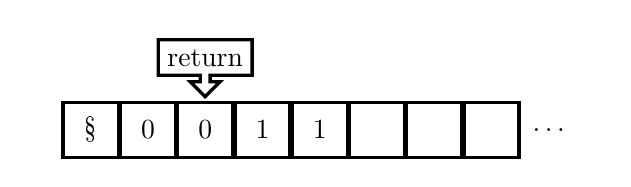
\begin{tikzpicture}
    \edef\sizetape{0.7cm}
    \tikzstyle{tmtape}=[draw, very thick,minimum size=\sizetape]
    \tikzstyle{tmhead}=[arrow box,draw, very thick, minimum width =.6cm,
                        arrow box arrows={south:.25cm}]

    % Draw TM tape
    \begin{scope}[start chain=1 going right,node distance=-0.15mm]
        \node [on chain=1,tmtape] {\S};
        \node [on chain=1,tmtape] {0};
        \node [on chain=1,tmtape] (input) {0};
        \node [on chain=1,tmtape] {1};
        \node [on chain=1,tmtape] {1};
        \node [on chain=1,tmtape] {};
        \node [on chain=1,tmtape] {};
        \node [on chain=1,tmtape] {};
        \node [on chain=1,tmtape,draw=none] {$\ldots$};
    \end{scope}
    \clip (-.8, -0.2) rectangle (6.5, 1.3);

    % Draw TM head below (input) tape cell
    \node [tmhead,yshift=.55cm] at (input.north) (head) {return};
  \end{tikzpicture}
\end{document}
